 
\documentclass[11pt]{article}
\usepackage[top=1in, bottom=1in, left=0.5in, right=0.5in]{geometry} 
\usepackage{graphicx}

\begin{document}
\title{CS296 group project, JCB digger, Group 26}
\author{Rakesh Ranjan Nayak\\
  120050047,\\
  \texttt{rakeshranjan@cse.iitb.ac.in}
  \and
  Amol Agarwal,\\
  120110031,\\
  \texttt{amola@cse.iitb.ac.in}
  \and 
  Shashank B, \\
  120050076, \\
  \texttt{shashankb@cse.iitb.ac.in}
  }
    
\date{\today}
\maketitle

\section{Introduction}
In this report we will go through our project details for CS296. We are simulating JCB digger in a rough terrain as our final project. We have used
Box2D Physics Engine for the simulation. We will be discussing various aspects of our project and what makes our project interesting. We will analyze 
profiling data related to our project and try to optimize our code based on the profiling data.

\section{Design for the complex machine}
The Initial design for the project is the figure below. We had thought of crawler JCB digger as our project idea. As there are Many joints in the machine
which work independently to give the digger it's behaviour, it is an example of complex machine.
\begin{center}
	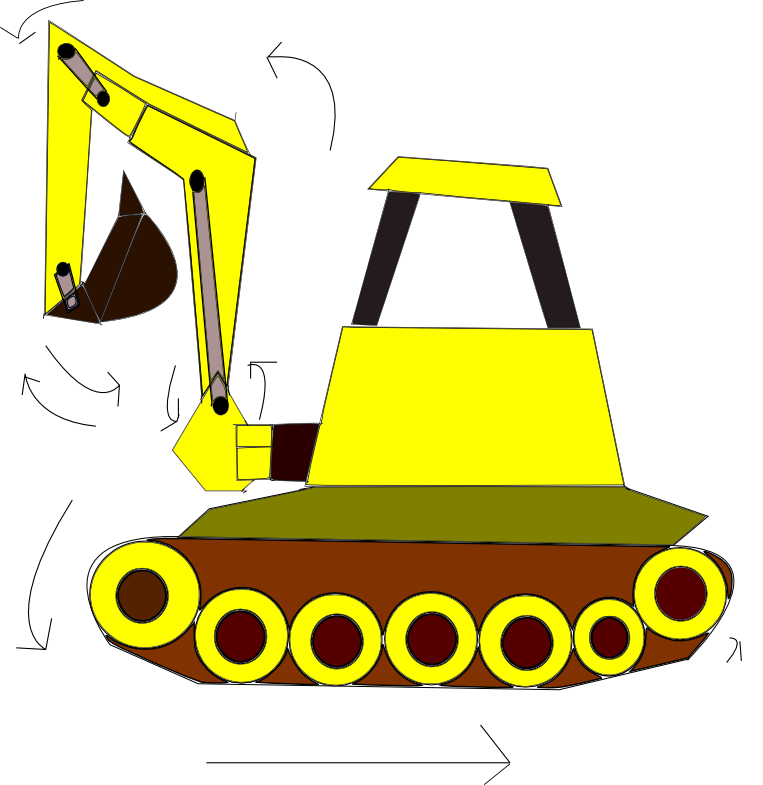
\includegraphics[scale=0.5]{images/drawing}
\end{center}	
We have tried to follow the design as close as possible though we deviated in some aspects. In our finished design we have omitted the track chain in the 
wheel and made the final design to resemble more like a JCB digger by having large wheels. We have added digger at the front of the machine which is controlled 
by varying piston compression attached to it. The machine is simulated in the environment using keyboard callbacks which changes the motorspeed of various 
joints in the machine.
\begin{center}
	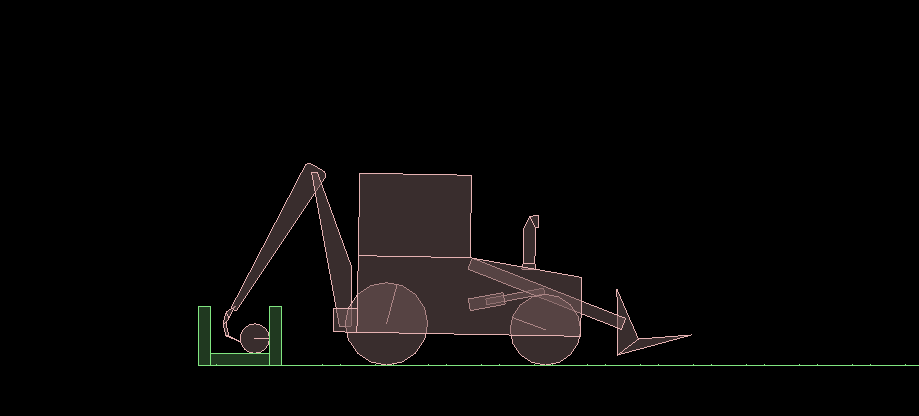
\includegraphics[scale=0.5]{images/final_design}
\end{center}
We have used random uneven terrain in our simulation. The machine needs to pick things up from the ground and put it inside the bins provided at the end 
of the track.The realistic design of the machine and the innovative idea to simulate our machine in Box2D makes our project interesting.
\begin{center}
	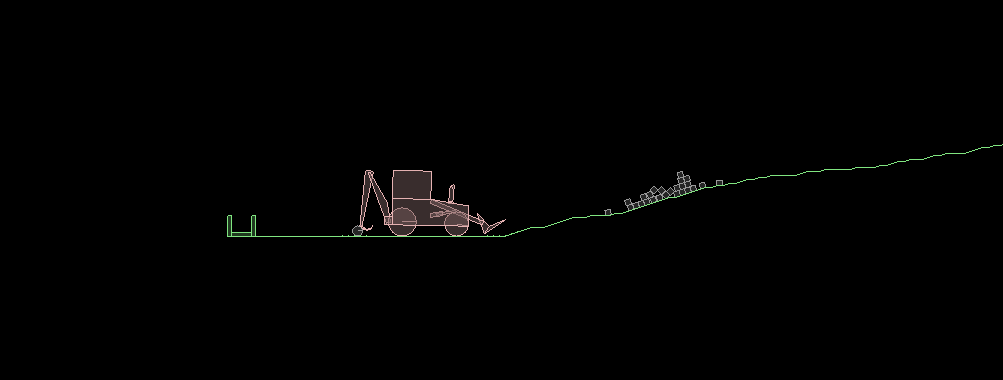
\includegraphics[scale=0.5]{images/final_design2}
\end{center}

\section{Graph analysis}
We simulated our design without GUI by removing all calls to GLUI and GLUT \cite{lab05}. In the main function, We calculated the average of many quantities like 
step time, collision update time, velocity update time and position update time based on the profile of m$\_$world imported from $base\_sim\_t$.
Based on the data received from the world profile we plotted graphs showing the relationship between many quantities like step time vs iteration etc. 
using Gnuplot and Matplotlib\cite{lab09}. As Matplotlib graphs are more clear, we considered showing them. We will try to explain the variations in the graphs
by simulating the environment again by adding GUI. \\
We plotted the graphs first by simulating our machine with even terrain for 150 iterations and 15 reruns. Then we gave random uneven terrain and 
placing obstacles at random locations in each rerun which we generated by seeding rand value to time at the moment. Then we removed the $srand()$ 
function call, and ran our source code for 1200 iterations and 150 reruns to get a good view of what is actually happening as the terrain is uneven 
now but not random. We gave some initial motor speed to wheels and other joints so that it will simulate automatically without keyboard callbacks.

	\subsection{Step time and loop time vs Number of Iterations} 
	The loop time is the total time for the `for' loop for ``iteration number" counts, therefore it increases almost lineary with iteration number 
	with slight variation in between. As it is generated using getTimeOfDay() function, it depends on other processes running at that point of time.
	As the avg. step time for various iteration counts are much smaller than that of avg. loop time in the later part of the graph, the plot for 
	avg. step time is not much clearer. 	
	\begin{center}
	  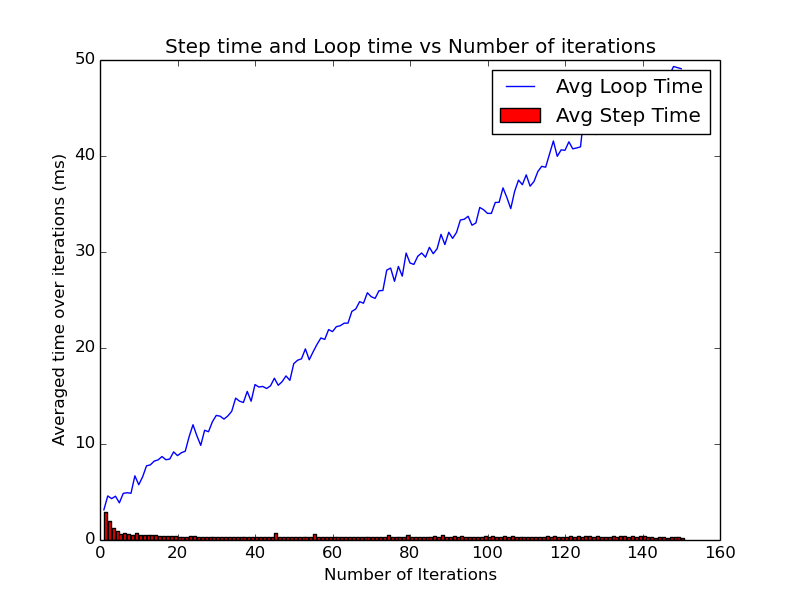
\includegraphics[scale=0.5]{images/g26_plot00_150x10_even}
	\end{center}
	\begin{center}
	  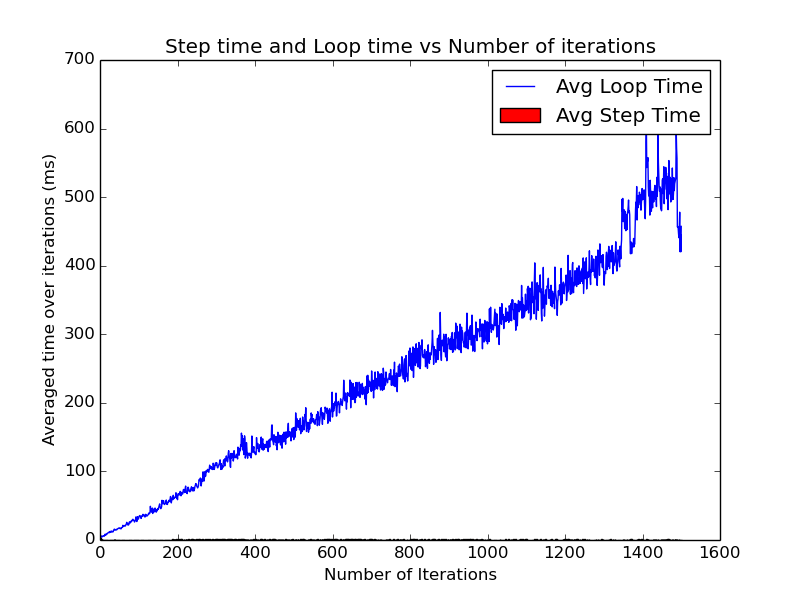
\includegraphics[scale=0.5]{images/g26_plot00_1500x10_random}
	\end{center}
	\begin{center}
	  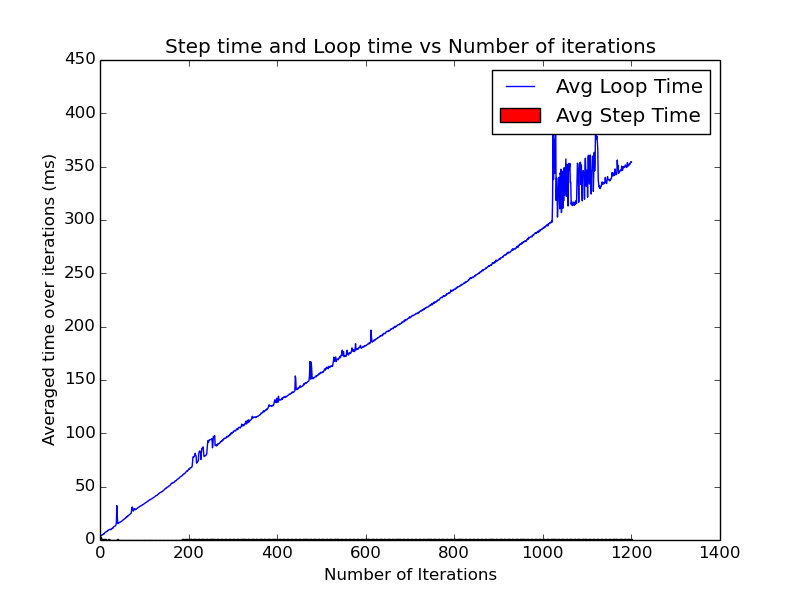
\includegraphics[scale=0.5]{images/g26_plot00_1200x150_uneven}
	\end{center}
	
	\subsection{Average step time, collision time, velocity time, position time and total time vs Number of Iterations} 
	The average step time, collision time ,velocity time ,position time and total time have almost similar profiles. Their values, on an average, decrease with 
	the number of iterations at first and at some points there are sudden variations in the graph which are produced by collision. The avg. step time  
	is more than the sum of avg. collision time, avg. velocity time and avg. position time throughout the graph. The variations are more in the data generated
	for random terrain. In the third plot, graph goes smooth upto 180 then variation occurs. This can be explained by change in the terrain which result in more 
	step times due to more position, velocity and collision updates.
	\begin{center}
	  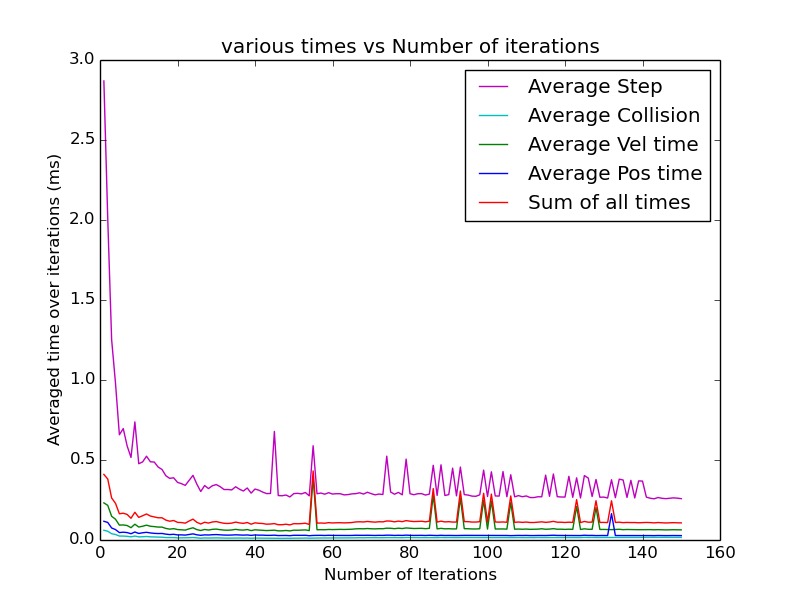
\includegraphics[scale=0.5]{images/g26_plot01_150x10_even}
	\end{center}	
	\begin{center}
	  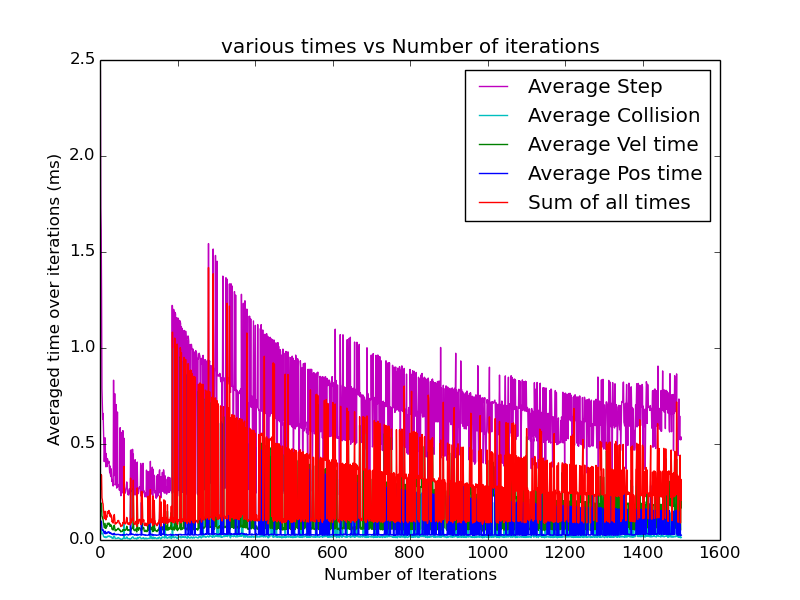
\includegraphics[scale=0.5]{images/g26_plot01_1500x10_random}
	\end{center}
	\begin{center}
	  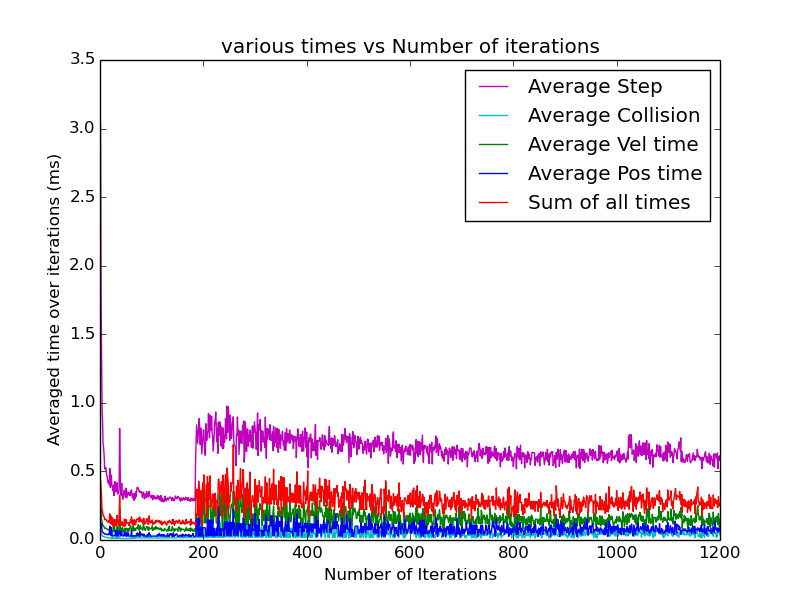
\includegraphics[scale=0.5]{images/g26_plot01_1200x150_uneven}
	\end{center}
	
	\subsection{Avg. step time with standard deviations vs iteration numbers} 
	The errors corresponding to greater step times are more than those of smaller step times. This can be explained by looking at the point graph of average 
	step time with iteration count as discussed later in the section. At the point of variation, some points lie far above other points in the graph which 
	result in greater avg. step time as well as more error.
	\begin{center}
	  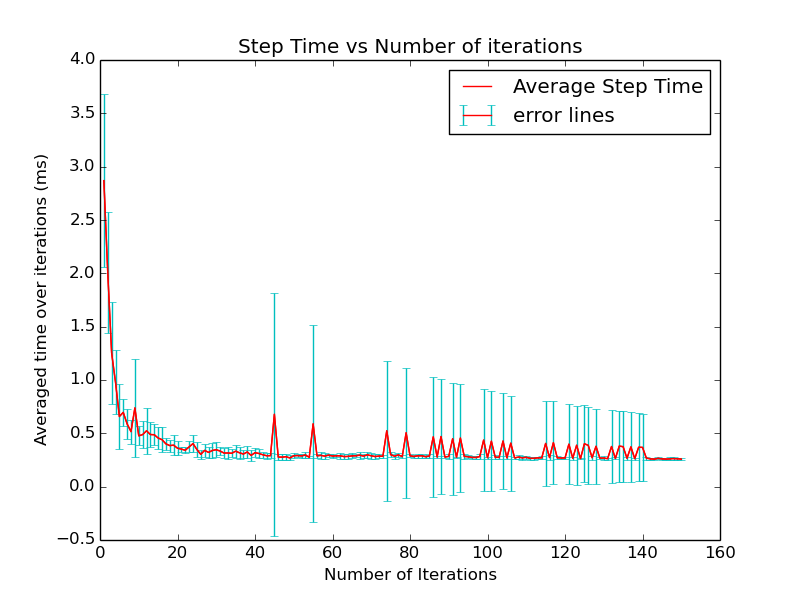
\includegraphics[scale=0.5]{images/g26_plot02_150x10_even}
	\end{center}
	\begin{center}
	  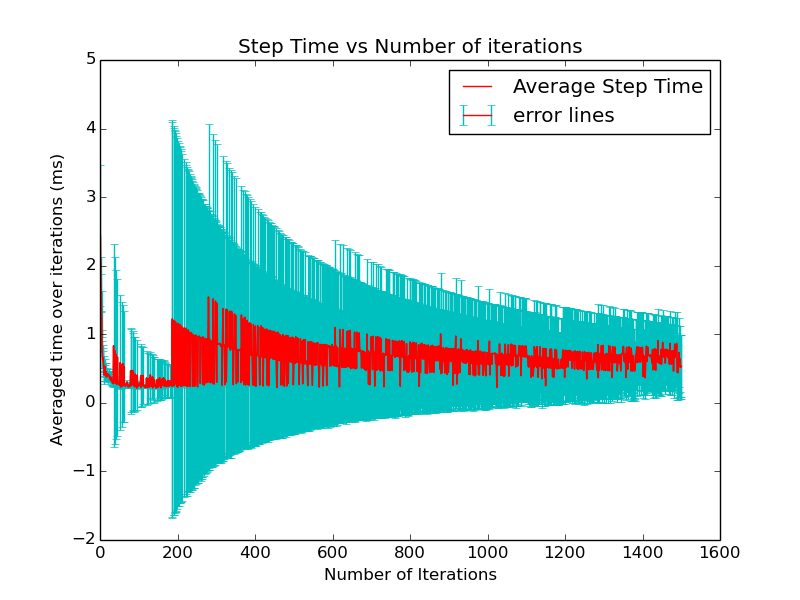
\includegraphics[scale=0.5]{images/g26_plot02_1500x10_random}
	\end{center}
	\begin{center}
	  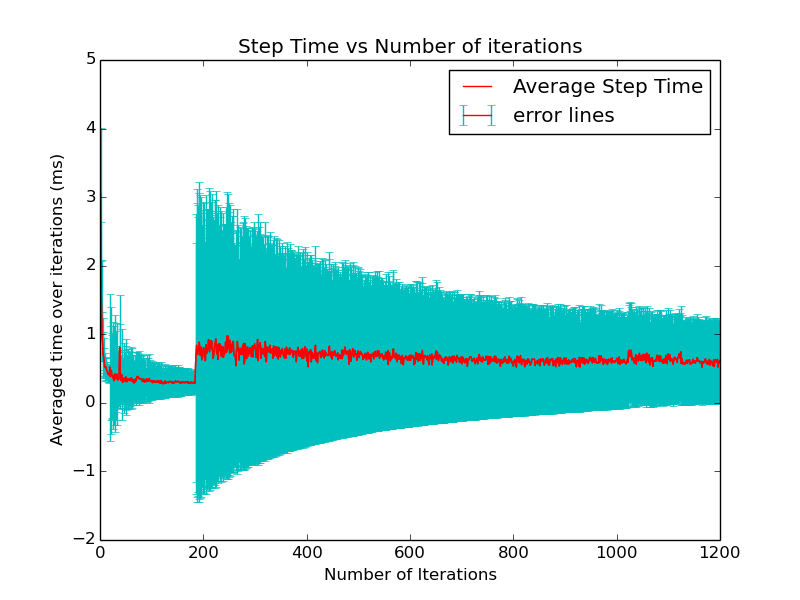
\includegraphics[scale=0.5]{images/g26_plot02_1200x150_uneven}
	\end{center}
	
	\subsection{Step Time Frequency Plot} 
	As is evident from the graph, for some small iteration count the distribution of step time is almost similar for both even terrain and random uneven terrain 
	because both terrains are even for some distance after which random terrain is created. The third graph shows that there are some points which lie far away 
	from their partners which result in more error.
	\begin{center}
	  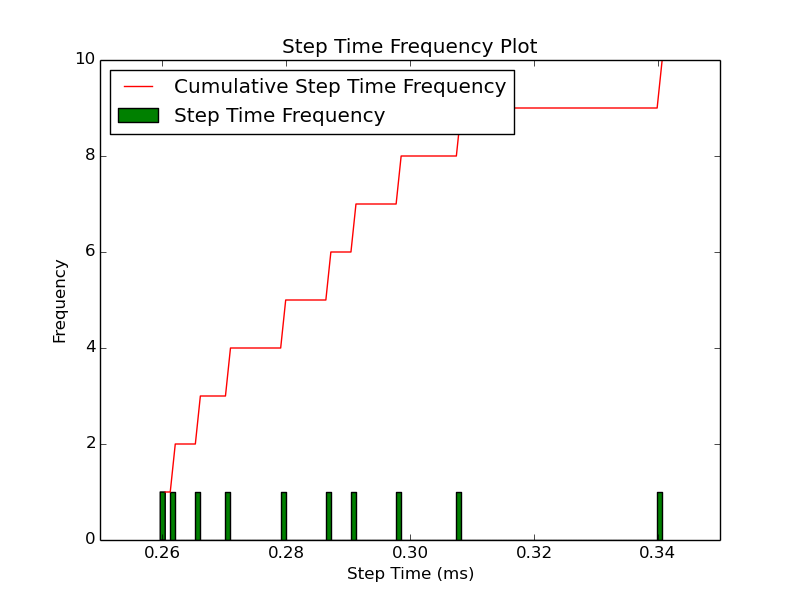
\includegraphics[scale=0.5]{images/g26_plot03_150x10_even}
	\end{center}
	\begin{center}
	  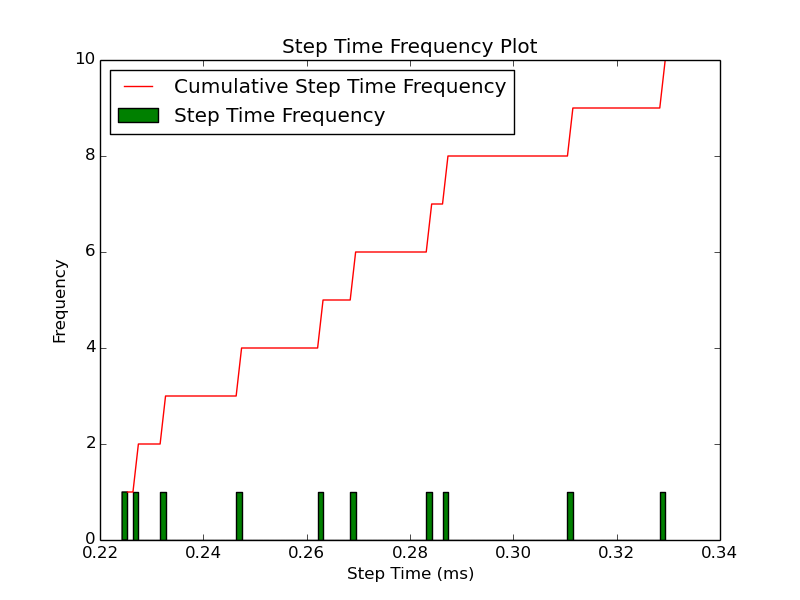
\includegraphics[scale=0.5]{images/g26_plot03_1500x10_random}
	\end{center}
	\begin{center}
	  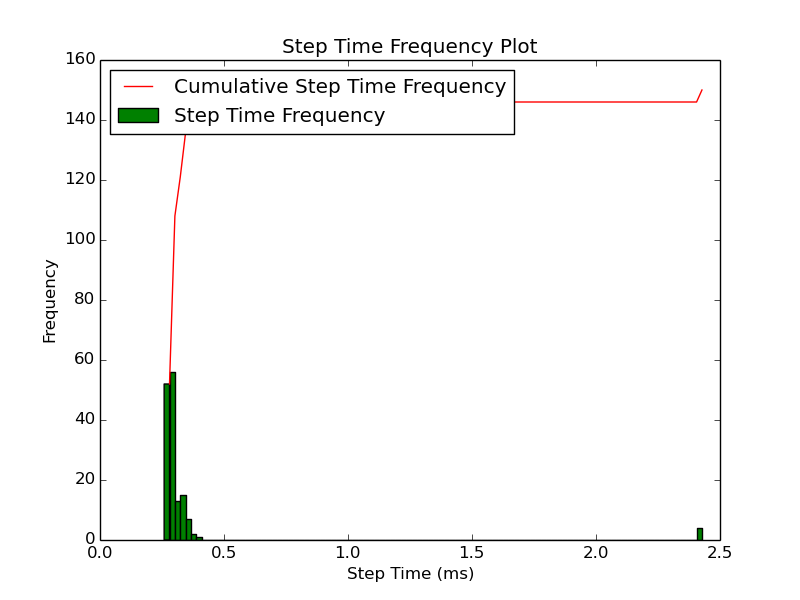
\includegraphics[scale=0.5]{images/g26_plot03_1200x150_uneven}
	\end{center}
	
	\subsection{step time vs number of iterations : point graph}
	For the first two graphs as the number of reruns per iteration is less than 15, We only plotted the point graph for step time of each rerun. Most of 
	the points in the first graph lie on a curve though at some points they deviate due to collision or extreme constraints. In the second graph, the points 
	form many curves  which can be explained by the fact that when segments change due to randomness in y1, the effective step time increases due to the 
	change in the terrain at the moment. As the value of y1 be -1 or 0, the curve would deviate at the intersection point if there is a change in y1. So, this 
	behaviour of the graph is expected.
	
	\begin{center}
	  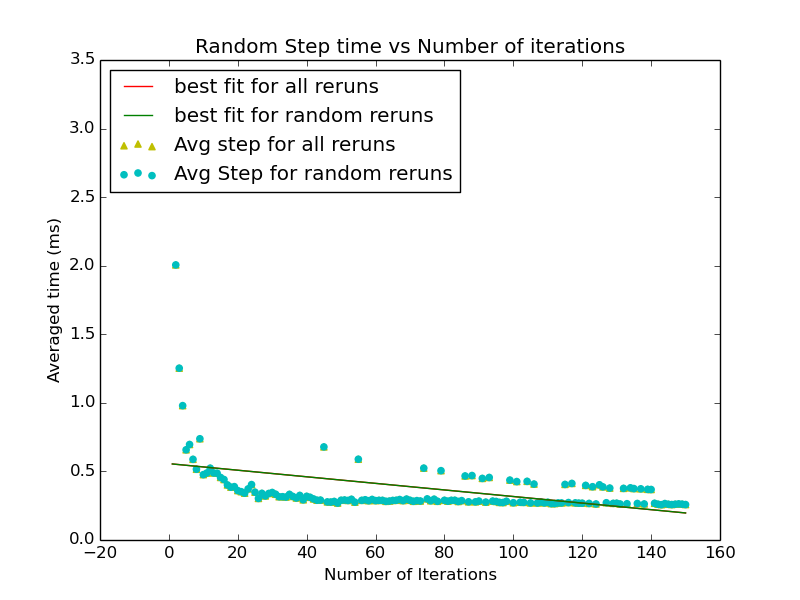
\includegraphics[scale=0.5]{images/g26_plot04_150x10_even}
	\end{center}
	\begin{center}
	  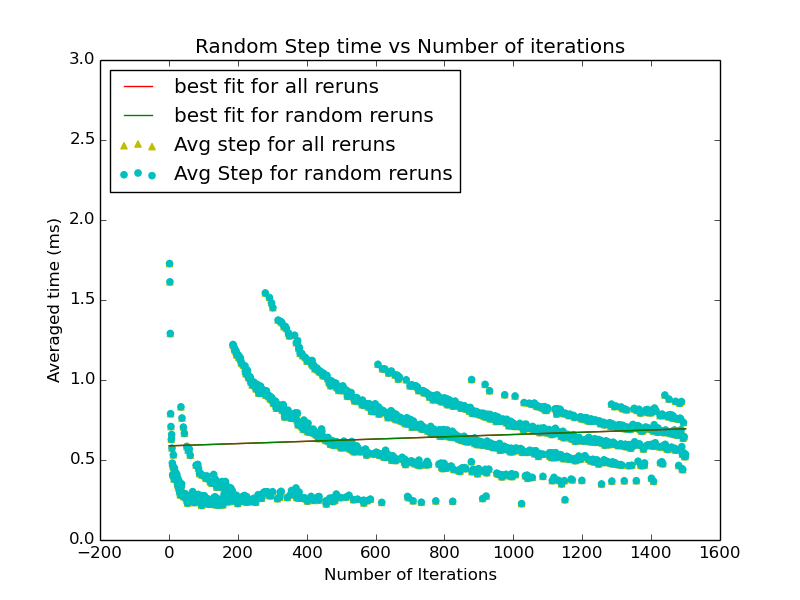
\includegraphics[scale=0.5]{images/g26_plot04_1500x10_random}
	\end{center}
	\begin{center}
	  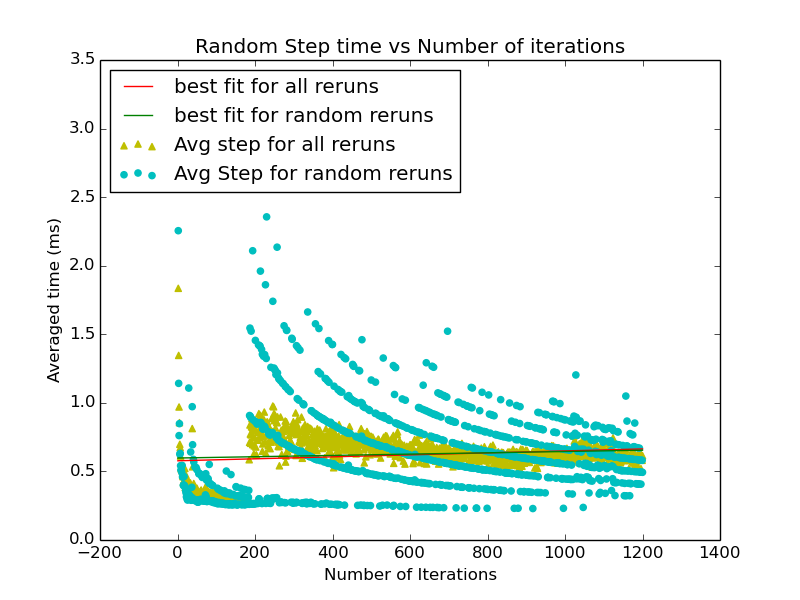
\includegraphics[scale=0.5]{images/g26_plot04_1200x150_uneven}
	\end{center}
	
\section{Callgraph analysis}
The callgraph is generated using gprof2dot.py \cite{lab07} python script after profiling the code using perf \cite{lab07}. The following inference are made based on the callgraph.
	\subsection{Nodes}
	It contains information regarding function names along with their namespaces, percentege of total time spent in the function
	(including all its children), self-time of thhe function, and total number of calls of that function.
	\subsection{Edges}
	It goes from a parent function to a child function.It is indicated by Number of calls that parent makes to child and percentage of 	time that is
	transferred to that child.
	\subsection{Analysis}
	$98.75\% $ of the time is spent in $cs296::base\_sim\_t()$ out of which $19.70\%$ is spent in creating graphics and $78.66\%$ is spent in $b2World::step()$
	function. $b2World::SolveTOI()$ takes $14.04\%$, $b2World::solve()$ takes $57.93\%$ , $b2ContactManager::collide()$ takes $6.06\%$ of the total time. 
	\begin{center}
		  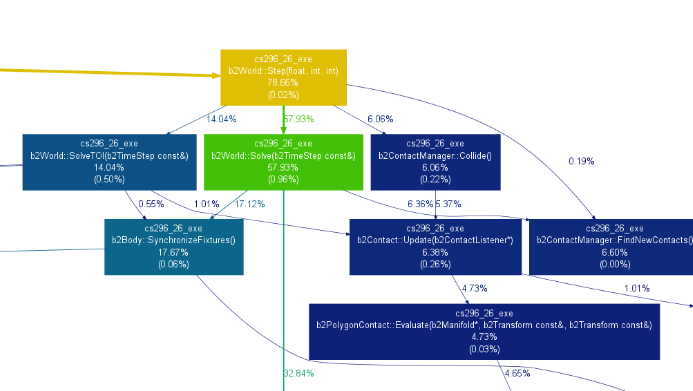
\includegraphics[scale=0.60]{images/b2World_step}
	\end{center}
	Out of the total $19.72\%$ time spent in $b2World::DrawDebugData()$, $17.67\%$ of the total time is spent in drawing shapes in the function
	$b2World::DrawShape().$
	\begin{center}
		  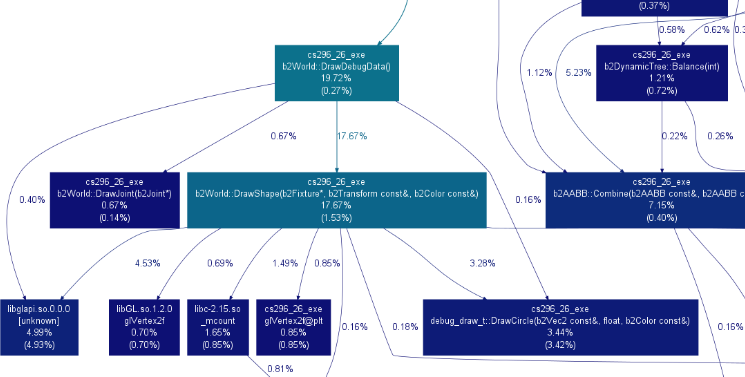
\includegraphics[scale=0.60]{images/DrawDebugData}
	\end{center}
	$32.84\%$ of the time is spent in $b2Island::solve()$ which calls various functions to solve Position and Velocity Constraints. Notable function calls
	are $b2RevoluteJoint::SolveVelocityConstraints()$, $b2RevoluteJoint::SolvePositionConstraints()$, $b2ContactSolver::SolveVelocityConstraints()$,
	$b2ContactSolver::SolvePositionConstraints()$ etc. In general, Velocity constraint solver functions take approx. double the time taken by Position Solver 
	functions.
	\begin{center}
		  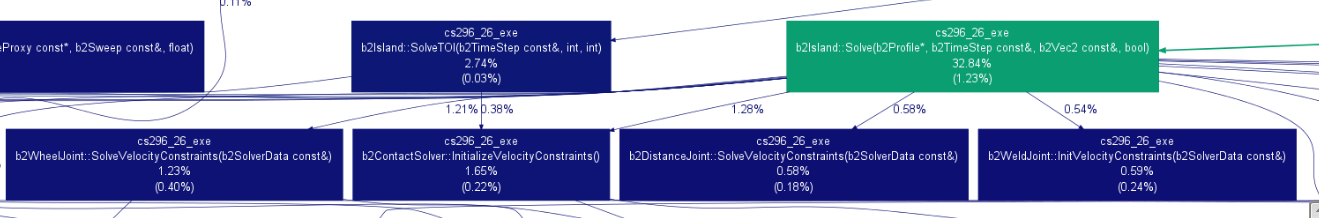
\includegraphics[scale=0.40]{images/b2Island_solve}
	\end{center} 

\section{Conclusion}
In this report we discussed about the profiling details for our project, what we did to optimize our code and \\
analysis of the performance of our project simulation using various graph plotting technique. We presented \\
our original design as well as finished design for the complex machine. We talked about many aspects  which makes \\ 
our project interesting.

\begin{thebibliography}{2}
	\bibitem{lab05}
	  Bash shell scripting and gnuplot,
	  Lab 05, CS296,
	  Parag Choudhari
	\bibitem{lab07}
	  Timing and profiling code,
	  Lab07, CS296 ,
	  Parag Choudhari
	\bibitem{lab09}
	  Python Programming,
	  Lab 08 and 09, CS296,
	  Parag Choudhari
	   

\end{thebibliography}
\end{document}
